\chapter{Implementación del modelo}
Este capítulo está dedicado a cubrir los detalles de la implementación del modelo en código, concretamente en lenguaje C++.

Dado que la principal finalidad de este trabajo es el modelado físico, no entraré en detalles en otras áreas del programa más que las que tienen que ver con lo descrito en los capítulos anteriores.

El programa completo contiene módulos para la graficación en \href{http://www.opengl.org/}{OpenGL}, para la interfaz de usuario por medio de \href{https://github.com/ocornut/imgui}{dear imgui}, para la lectura y escritura de imágenes usando \href{http://freeimage.sourceforge.io/}{freeimage} (para cargar texturas y para hacer capturas de pantalla) e implementa el modelo de iluminación de \href{http://en.wikipedia.org/wiki/Phong_reflection_model}{Phong} en shaders por medio de \href{http://www.khronos.org/opengl/wiki/OpenGL_Shading_Language}{GLSL}.

El lector interesado puede consultar el código fuente completo del programa que se incluye en un CD o puede descargarlo de \href{http://github.com/nemediano}{github}.
Aunque el código está escrito en inglés (por ser el estándar) traté de ser lo más extenso en los comentarios en todo el código.
Por lo que el lector que cuente con los conocimientos de programación y graficación por computadora adquiridos en la licenciatura podrá entender y usar todo el código fuente del programa sin ningún problema.

Se decidió implementar el programa usando el paradigma de programación orientada a objetos. 
En la primera sección se describen las clases más importantes: las necesarias para representar las estructuras del modelo y la clase que representa el cuerpo neumático.

La siguiente sección se revisa cómo se implementaron en código los métodos numéricos usados para integrar la ecuación de Newton.

En la tercera sección se explican las rutinas de la física del modelo, concretamente las rutinas que se encargan de aplicar las fuerzas que intervienen en el modelo.

En la última sección del capítulo, se explica cómo es que se implementaron la rutina tanto de detección como de respuesta a las colisiones.

\section{Diseño de clases}

\epigraph{\say{Show me your flowchart and conceal your tables, and I shall continue to be mystified. Show me your tables, and I won't usually need your flowchart; it'll be obvious.}}{\textit{Frederick P. Brooks \\ Mythical Man-Month}}

Decidí usar de la biblioteca de álgebra para gráficos \href{http://github.com/g-truc/glm}{glm} por dos razones:
Primero, porque cuenta con tipos de datos para representar vectores en 2 y 3 dimensiones e implementa las operaciones usuales entre ellos.
Y segundo, porque esta biblioteca tiene un alto nivel de integración con OpenGL al grado de ser casi un estándar.

La parte fundamental del modelo la constituyen las partículas; de cada una de éstas nos interesa saber básicamente cuatro cosas: su posición, su velocidad, la fuerza que se le está aplicando y la masa.
Adicionalmente, por un detalle particular a nuestra implementación, se necesita saber si una partícula está fija.
Si una partícula está fija, entonces se deben de ignorar las operaciones de integración.
La clase \mintinline{cpp}{Particle} representa (abstrae) una partícula. Los métodos nos permiten editar y consultar estos cinco miembros.
En este sentido la clase \mintinline{cpp}{Particle} es muy simple~\footnote{En el argot del lenguaje \href{http://www.java.com/en/}{Java} diriamos que la clase \mintinline{cpp}{Particle} es casi un \href{http://en.wikipedia.org/wiki/JavaBeans}{bean}}.

Para representar a los resortes-amortiguadores se creó la clase \mintinline{cpp}{SpringDamper} que tiene como miembros \emph{referencias} a las dos partículas que une éste resorte.
Hago énfasis en que usaremos referencias, pues las partículas van ser usadas para formar varios objetos y se requiere que no sea necesario actualizar en cada objeto por separado cada que una partícula sea modificada. Finalmente, se debe saber la longitud $L$ del resorte cuando está en su estado de reposo.

La clase \mintinline{cpp}{SpringDamper} define los métodos para:
\begin{itemize}
 \item Actualizar qué partículas forman éste resorte.
 \item Consultar y modificar $L$.
 \item Consultar las posiciones de las partículas que forman éste resorte.
 \item Acumular la fuerza del resorte en sus dos partículas dados $k_s$ y $k_d$.
\end{itemize}

La última clase necesaria para definir el cuerpo neumático es la clase \mintinline{cpp}{Face}, que representa una cara del cuerpo flexible.
Como es de esperar, dado que las caras son cuadriláteros, esta clase solo necesita como propiedades referencias a cuatro partículas.

Adicionalmente, la clase \mintinline{cpp}{Face} implementa los siguientes métodos:
\begin{itemize}
 \item Los accesores y mutadores a las partículas que la forman.
 \item Un método para actualizar las partículas que forman esta cara (equivalente al de \mintinline{cpp}{SpringDamper}).
 \item Un método para calcular el área de esta cara.
 \item Un método que sirve como auxiliar en el cálculo del volumen de todo el cuerpo flexible. La lógica de este método se explica en la Sección~\ref{sec:fuerzaGas}.\footnote{Aunque ésta no es estrictamente hablando una propiedad de la cara, por razones de Ingeniería de Software (IS) era conveniente incluirlo en esta clase.}
\end{itemize}

La clase que representa el cuerpo flexible: \mintinline{cpp}{SoftBody} está compuesta con objetos de las clases anteriores.
Esta clase es la más importante de la aplicación.
Y el resto de éste capítulo está dedicado a explicar como funcionan sus métodos.
En este momento, es relevante decir que esta clase contiene una colección de partículas, una colección de resortes y una colección de caras.
Las caras y resortes en realidad usan (agregan) referencias a las partículas, de esta manera la información de las partículas sólo está almacenada una vez.

Por orden, esta clase también define una estructura: \mintinline{cpp}{SoftBodyParameters} que contiene todos los parámetros físicos del cuerpo flexible. 
 
Finalmente, se necesita también una clase para representar el único cuerpo rígido en la escena.
La clase \mintinline{cpp}{Ball} tiene como miembros una partícula, un escalar que representa el radio de la esfera y un miembro para registrar qué método numérico se usa para integrar.\footnote{De nuevo por IS, era conveniente que cada objeto en la escena llevará registro de que integrador está en uso}

La relación entre estas clases está resumida en el diagrama de clases mostrado en la Figura~\ref{clases:fig}. De nuevo hago énfasis en que la implementación de contiene de hecho más miembros que los mostrados en dicha figura, pues solo aparecen en el diagrama los relevantes para éste trabajo.

\begin{figure}
 \centering
 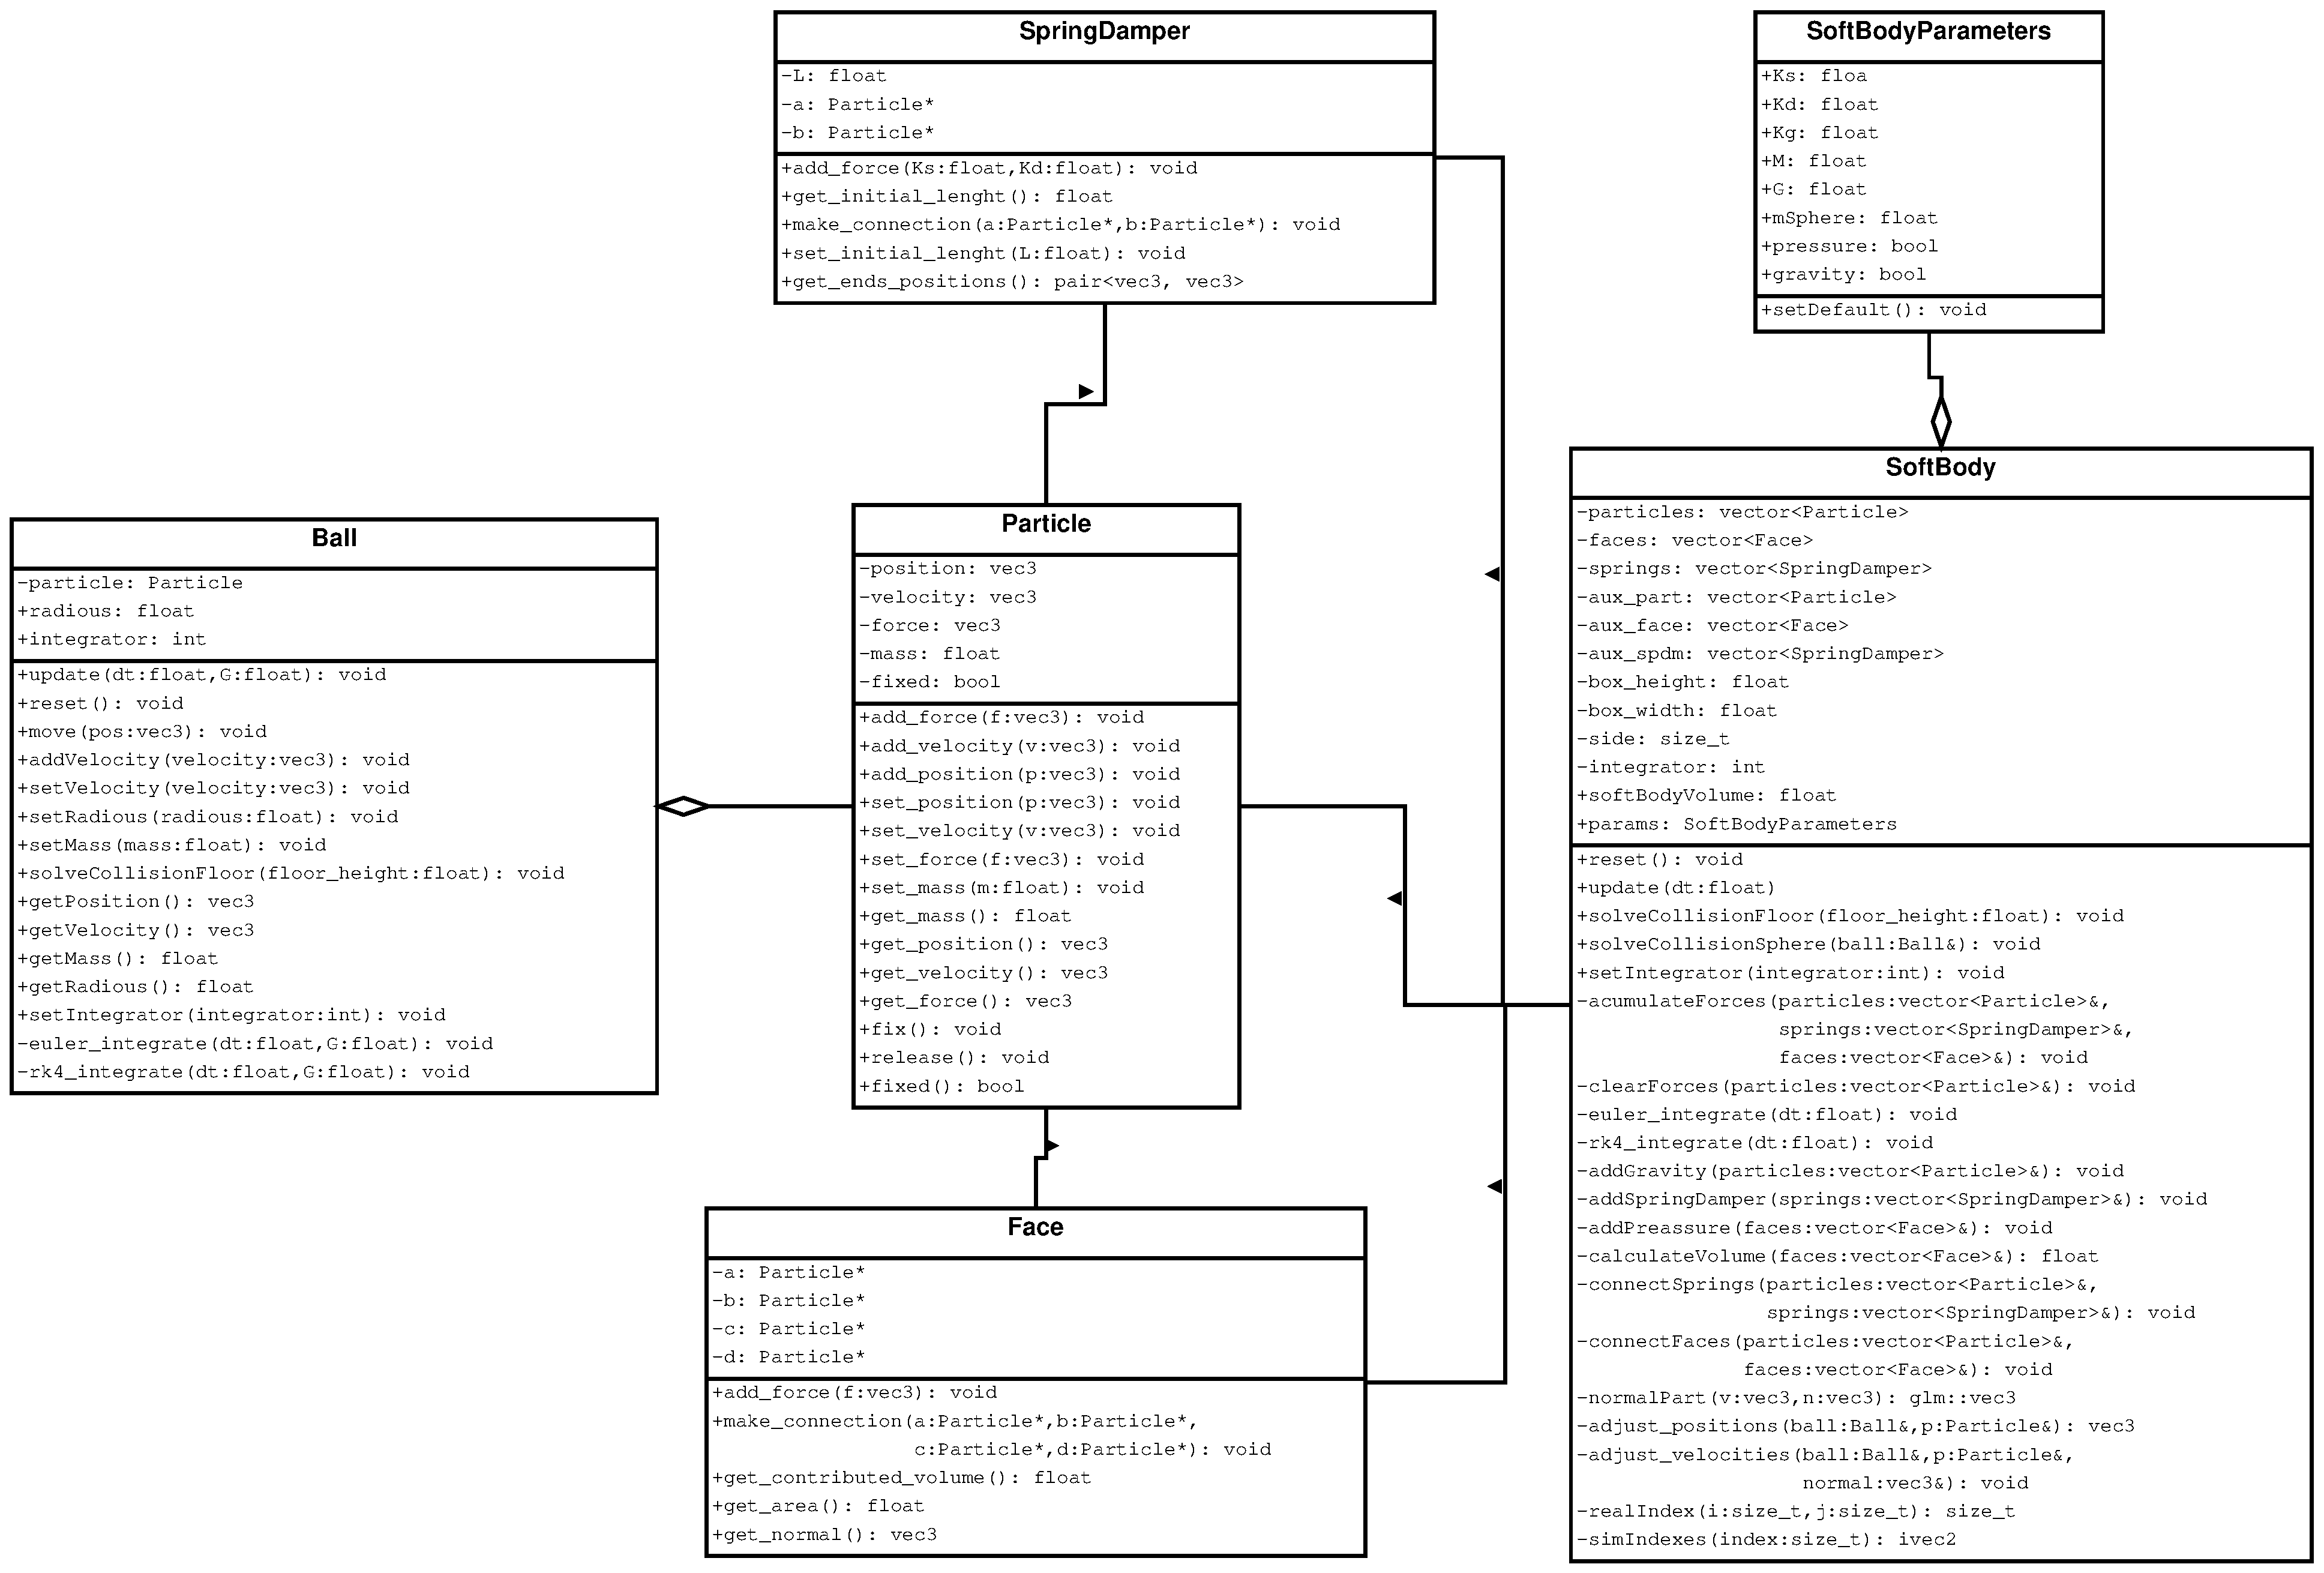
\includegraphics[width=\textwidth]{Img/03/diagramaClases}
 \caption[Diagrama de clases]{ 
 La clase \mintinline{cpp}{Particle} es la unidad de construcción. La clase \mintinline{cpp}{SoftBody} es el objeto principal que contiene a los demas. 
 } \label{clases:fig}
\end{figure}

\section{Creación del cuerpo flexible}

Cómo se dijo en la sección anterior, hay tres colecciones que forman el cuerpo flexible: las partículas, los resortes y las caras.
Estas colecciones están almacenadas en arreglos dinámicos\footnote{En lenguaje C++ representados por objetos de tipo \mintinline{cpp}{std::vector}, los llamo \emph{colecciones} en el texto para no confundirlos con los vectores de álgebra lineal} que forman parte de la clase \mintinline{cpp}{SoftBody}.

Hay algunas cosas que decir aquí: primero, que lo que se quiere modelar es una tela cuadrada que servirá como cuerpo flexible, por lo que el número de partículas es en realidad $n^{2}$ en donde $n$ es el número de puntos en cada lado de la tela (en el código, $n$ es el miembro \mintinline{cpp}{m_side} de \mintinline{cpp}{SoftBody}), y como no hay resortes en las orillas de la tela el número de resortes totales es $2 (n - 1) (n - 2)$ y el número de caras es: $(n-1)^{2}$.
Segundo, que pese a que geométricamente la tela es un arreglo cuadrado de puntos, las partículas son guardados en un arreglo unidimensional (lineal), dado que esto  simplifica y hace mucho más generales las rutinas de acumulación de fuerza.

Dado que la partículas están en un arreglo unidimensional se hace uso del método \mintinline{cpp}{simIndexes} que recibe el índice de la partícula en el vector unidimensional y nos regresa los índices $(i, j)$ que la partícula tendría en un arreglo bidimensional. El método \mintinline{cpp}{realIndex} hace la operación inversa.

\begin{listing}
\inputminted[
  firstline=303, %If you omit this two fields, the whole file is pulled
  lastline=341
  ]{cpp}{../../../GLSamples/SoftBody/physics/SoftBody.cpp}
  \caption{El método \mintinline{cpp}{recreate_particles} de \mintinline{cpp}{SoftBody}}\label{lst:recreate_particles}
\end{listing}

El código mostrado en el Listado~\ref{lst:recreate_particles} inicializa la velocidad, la fuerza y la masa de la partículas (la posición es inicializada con una rutina muy simple que está fuera de la clase \mintinline{cpp}{SoftBody}). 
También se encarga de fijar las partículas que están en las orillas de la tela.

La rutina que inicializa los resortes es ejecutada después que la de las partículas. Se muestra un extracto en el Listado~\ref{lst:connectSprings}.

\begin{listing}
\inputminted[
  firstline=343, %If you omit this two fields, the whole file is pulled
  lastline=371
  ]{cpp}{../../../GLSamples/SoftBody/physics/SoftBody.cpp}
  \caption{El método \mintinline{cpp}{connectSprings} de \mintinline{cpp}{SoftBody}}\label{lst:connectSprings}
\end{listing}

Por las condiciones que definimos en nuestra tela.
\begin{itemize}
 \item Las partículas que están en las aristas superiores e inferiores de la tela no tienen un resorte horizontal entre ellas.
 \item Las partículas que están en las aristas izquierda y derecha de la tela no tienen un resorte vertical entre ellas.
\end{itemize}

El algoritmo, pregunta si esta partícula puede ser unida (por un resorte) con la partícula a su derecha, de ser así las conecta. Después, pregunta si debe ser unida con la partícula debajo de ella, de ser así también es conectada.

\begin{listing}
\inputminted[
  firstline=373, %If you omit this two fields, the whole file is pulled
  lastline=392
  ]{cpp}{../../../GLSamples/SoftBody/physics/SoftBody.cpp}
  \caption{El método \mintinline{cpp}{connectFaces} de \mintinline{cpp}{SoftBody}}
  \label{lst:connectFaces}
\end{listing}

La lógica para formar las caras se presenta en el Listado~\ref{lst:connectFaces}.
Esta rutina es muy parecida a la anterior: recorre todas las partículas, si la partícula actual, tiene un partícula a su izquierda y otra partícula abajo, entonces se pueden tomar cuatro partículas (pues debe existir otra una partícula en diagonal) para formar una cara.

\section{La física del modelo}
Toca el turno de ver las rutinas que tienen que ver con la acumulación de fuerzas en el modelo.
Como se ha dicho antes hay básicamente tres fuerzas que se deben acumular, la de la gravedad, la de los resortes amortiguadores y la debida a la presión del gas.

Aquí es donde empezaremos a notar el porqué de la construcción de los demás vectores de referencias.

\subsection{La fuerza de gravedad}
La primera y más sencilla de las fuerzas que vamos a poner es la de gravedad.
Como se dijo desde la ecuación~\eqref{fuerzaGravedad}, sólo depende de dos cosas de la masa del objeto y de la constante de gravedad\footnote{La contribución de la masa será \emph{cancelada} por el integrador}, y además sólo afecta el componente vertical (paralelo al eje $y$), del vector fuerza.

La fuerza de gravedad se aplica a cada una de las partículas del cuerpo flexible. 
Convenientemente, tenemos un vector con dichas partículas.
Por lo anterior y gracias a que glm sobrecarga los operadores en vectores de la manera natural, la implementación es trivial como se puede ver en el Listado~\ref{lst:addGravity}.
La constante de gravedad es un miembro de \mintinline{cpp}{SoftBody} y tiene el signo negativo.

Para hacer posible el analisis de la Sección~\ref{sec:performance}, se hacen uso de cronómetros. La estructura \mintinline{cpp}{mTimers} contiene estos cronómetros  y el Listado~\ref{lst:addGravity} es un claro ejemplo de su uso. Estos cronómetros son una forma muy simplista de \emph{instrumentación} de un método.

\begin{listing}
\inputminted[
  firstline=589, %If you omit this two fields, the whole file is pulled
  lastline=598
  ]{cpp}{../../../GLSamples/SoftBody/physics/SoftBody.cpp}
  \caption{El método \mintinline{cpp}{addGravity} de \mintinline{cpp}{SoftBody}}
  \label{lst:addGravity}
\end{listing}

\subsection{La fuerza de los resortes}

La implementación de estos métodos también es trivial gracias a nuestro diseño.
Tan solo se debe iterar por todos los resortes de \mintinline{cpp}{SoftBody} en cada resorte se debe ocupar la ecuación~\eqref{fuerzaResorte}, para acumular la fuerza en los dos puntos que son unidos por ese resorte (Listado~\ref{lst:addSpringDamper}).
Solo por completez, en Listado~\ref{lst:add_forceSD} se muestra el método \mintinline{cpp}{add_force} de \mintinline{cpp}{SpringDamper} que en esencia implementa la ecuación~\eqref{fuerzaResorte}.

\begin{listing}
\inputminted[
  firstline=600, %If you omit this two fields, the whole file is pulled
  lastline=607
  ]{cpp}{../../../GLSamples/SoftBody/physics/SoftBody.cpp}
  \caption{El método \mintinline{cpp}{addSpringDamper} de \mintinline{cpp}{SoftBody}}
  \label{lst:addSpringDamper}
\end{listing}

\begin{listing}
\inputminted[
  firstline=19, %If you omit this two fields, the whole file is pulled
  lastline=32
  ]{cpp}{../../../GLSamples/SoftBody/physics/SpringDamper.cpp}
  \caption{El método \mintinline{cpp}{add_force} de \mintinline{cpp}{SpringDamper}}
  \label{lst:add_forceSD}
\end{listing}

\subsection{La fuerza del gas}
\label{sec:fuerzaGas}

La siguiente fuerza en ser acumulada es la fuerza debida a la presión del gas. Para esto se ocupa la ecuación~\eqref{fuerzaGas}, y se debe de acumular en cada cara.
Para poder calcular esta fuerza se necesitan hacer varias operaciones importantes: calcular el volumen total del cuerpo flexible y además calcular el área y el vector normal de cada una de las caras (Listado~\ref{lst:addPreassure}).

\begin{listing}
\inputminted[
  firstline=609, %If you omit this two fields, the whole file is pulled
  lastline=623
  ]{cpp}{../../../GLSamples/SoftBody/physics/SoftBody.cpp}
  \caption{El método \mintinline{cpp}{addPreassure} de \mintinline{cpp}{SoftBody}}
  \label{lst:addPreassure}
\end{listing}

Para hacer el cálculo de volumen se hace uso de la ecuación~\eqref{eq:volumen}.
Hay que recordar que el cuerpo neumático está formado por seis caras.
Cinco de las cuales están fijas y otra es la tela (o tapa) que es el cuerpo flexible.
Cada cara es dividida en dos triángulos para calcular su contribución al volumen.
El Listado~\ref{lst:calculateVolume} muestra la lógica. La función \mintinline{cpp}{tethVolume} implementa las ecuaciones~\eqref{eq:baricentro} y~\eqref{eq:normTriag} y por completez se muestra en el Listado~\ref{lst:calculateTethVolume}.

\begin{listing}
\inputminted[
  firstline=625, %If you omit this two fields, the whole file is pulled
  lastline=660
  ]{cpp}{../../../GLSamples/SoftBody/physics/SoftBody.cpp}
  \caption{El método \mintinline{cpp}{calculateVolume} de \mintinline{cpp}{SoftBody}}
  \label{lst:calculateVolume}
\end{listing}

\begin{listing}
\inputminted[
  firstline=35, %If you omit this two fields, the whole file is pulled
  lastline=41
  ]{cpp}{../../../GLSamples/SoftBody/math/mathhelpers.cpp}
  \caption{La función \mintinline{cpp}{tethVolume} implementa parte de la ecuación~\eqref{eq:volumen}}
  \label{lst:calculateTethVolume}
\end{listing}

El método \mintinline{cpp}{calculateVolume} de la clase \mintinline{cpp}{Face}, suma la contribución de una cara al volumen usando la misma función \mintinline{cpp}{tethVolume} dos veces en los puntos que forman la cara (Listado~\ref{lst:get_contributed_volume})

\begin{listing}
\inputminted[
  firstline=65, %If you omit this two fields, the whole file is pulled
  lastline=73
  ]{cpp}{../../../GLSamples/SoftBody/physics/Face.cpp}
  \caption{El método \mintinline{cpp}{get_contributed_volume} de \mintinline{cpp}{Face}}
  \label{lst:get_contributed_volume}
\end{listing}

Para calcular el área de cada cara se ocupa la fórmula~\eqref{formulaArea}, como se puede ver en el Listado~\ref{lst:get_area}.
Y para calcular el vector normal se hace uso de la fórmula~\eqref{formulaVecNormal}, en donde $n=4$, dado que cada cara está formada por cuatro puntos (Listado~\ref{lst:get_normal}).

\begin{listing}
\inputminted[
  firstline=44, %If you omit this two fields, the whole file is pulled
  lastline=53
  ]{cpp}{../../../GLSamples/SoftBody/physics/Face.cpp}
  \caption{El método \mintinline{cpp}{get_area} de \mintinline{cpp}{Face}}
  \label{lst:get_area}
\end{listing}

\begin{listing}
\inputminted[
  firstline=55, %If you omit this two fields, the whole file is pulled
  lastline=63
  ]{cpp}{../../../GLSamples/SoftBody/physics/Face.cpp}
  \caption{El método \mintinline{cpp}{get_normal} de \mintinline{cpp}{Face}}
  \label{lst:get_normal}
\end{listing}

\section{Los métodos numéricos}
Otras de las rutinas complicadas son los métodos numéricos.
Para integrar la ecuación de Newton, se requiere saber la posición y la velocidad actual de cada una de las partículas del modelo y tener una manera de llamar a la función que se encarga de acumular las fuerzas.

\subsection{El método de Euler}
Básicamente se trata de tomar las ecuaciones~\eqref{formulas:Euler} e implementarlas en el código (Listado~\ref{lst:euler_integrate}), aprovechando la gran ventaja de que el método de Euler puede integrar una partícula la vez.

\begin{listing}
\inputminted[
  firstline=466, %If you omit this two fields, the whole file is pulled
  lastline=477
  ]{cpp}{../../../GLSamples/SoftBody/physics/SoftBody.cpp}
  \caption{El método \mintinline{cpp}{euler_integrate} de \mintinline{cpp}{SoftBody}}
  \label{lst:euler_integrate}
\end{listing}

\subsection{El método de Runge-Kutta}
Aquí se explica el que fue probablemente el método numérico más complicado de implementar, pues no tiene la ventaja de Euler de integrar cada partícula independientemente, así que necesita integrar todas juntas.
Además, debe tener espacio para guardar los ponderadores del paso de integración de cada partícula.

Para tener una idea clara de lo que que hace el código en el Listado~\ref{lst:rk4_integrate} conviene volver a ver las ecuaciones~\eqref{ponderadores:RK4} y~\eqref{formulas:RK4}.
Lo largo del proceso hacen ver el Listado~\ref{lst:rk4_integrate} un poco más complicado que lo que en realidad es.

\begin{mintedCode} %El codigo es muy largo, ocupo un ambiene no flotante
\inputminted[
  firstline=479, %If you omit this two fields, the whole file is pulled
  lastline=556
  ]{cpp}{../../../GLSamples/SoftBody/physics/SoftBody.cpp}
  \caption{El método \mintinline{cpp}{rk4_integrate} de \mintinline{cpp}{SoftBody}}
  \label{lst:rk4_integrate}
\end{mintedCode}

El truco consiste en ocupar un conjunto de puntos, resortes y caras auxiliares, para con ellos evaluar la función fuerza que es necesaria para calcular los ponderadores del método de RK4 (Por eso están presentes en el diagrama de la Figura~\ref{clases:fig}), después la rutina es muy parecida a la de Euler.

\section{El manejo de las colisiones}
Como ya se ha dicho antes, el problema de las colisiones se resuelve en dos partes: primero la detección y luego la respuesta.
La forma de responder consiste básicamente en mover los objetos que se colisionan a un lugar donde ya no choquen y ajustar las velocidades como respuesta.

\subsection{La rutina de las colisiones}
La detección es llevada a cabo en dos funciones.
Recordemos que nuestra tarea de detección se simplifica muchísimo por el hecho de que uno de los objetos, el objeto incidente es una esfera.
Para saber si dicha esfera está en colisión con nuestro cuerpo flexible, lo que hacemos es probar si cualquiera de las partículas está dentro de la esfera; de ser así, empezamos a resolver la colisión entre la esfera y la partícula en cuestión. Después seguimos revisando el resto de las partículas.
El Listado~\ref{lst:solveCollisionSphere} implementa el algoritmo.

\begin{listing}
\inputminted[
  firstline=700, %If you omit this two fields, the whole file is pulled
  lastline=713
  ]{cpp}{../../../GLSamples/SoftBody/physics/SoftBody.cpp}
  \caption{El método \mintinline{cpp}{solveCollisionSphere} de \mintinline{cpp}{SoftBody}}
  \label{lst:solveCollisionSphere}
\end{listing}

\subsection{La detección de la colisión}
El método del Listado~\ref{lst:adjust_positions} en se encarga de calcular el vector normal al lugar de la colisión y de mover el punto fuera de la esfera.
Mover el punto fuera de la esfera es en realidad parte de la respuesta a la colisión, pero decidí implementarlo en un solo método llamado \mintinline{cpp}{adjust_positions}, para que en la siguiente parte sólo se tenga que ajustar las velocidades.

\begin{listing}
\inputminted[
  firstline=715, %If you omit this two fields, the whole file is pulled
  lastline=728
  ]{cpp}{../../../GLSamples/SoftBody/physics/SoftBody.cpp}
  \caption{El método \mintinline{cpp}{adjust_positions} de \mintinline{cpp}{SoftBody}}
  \label{lst:adjust_positions}
\end{listing}

El Listado~\ref{lst:adjust_positions}, primero calcula el vector normal que va del centro de la esfera a la partícula.
Luego, si la partícula no está fija, la mueve justo fuera de la esfera.
Si la partícula estuviera fija, lo que hace es mover a la esfera fuera de ella.

\subsection{La respuesta de la colisión}
La mayor parte del trabajo se hizo en la función anterior, ahora que sabemos el vector normal unitario: $\vec{\textbf{n}}$ a la colisión, el Listado~\ref{lst:adjust_velocities} solo se encarga de seguir los pasos explicados en el Algoritmo~\ref{alg:elasmov}.

\begin{listing}
\inputminted[
  firstline=730, %If you omit this two fields, the whole file is pulled
  lastline=745
  ]{cpp}{../../../GLSamples/SoftBody/physics/SoftBody.cpp}
  \caption{El método \mintinline{cpp}{adjust_velocities} de \mintinline{cpp}{SoftBody}}
  \label{lst:adjust_velocities}
\end{listing}

Es importante que la velocidad y posición de la esfera sean ajustadas de manera independiente por cada partícula con la que se haya producido una colisión.
Es \emph{físicamente incorrecto} tratar de acumular las posiciones y velocidades de respuesta de colisión con cada partícula y luego actualizar el cuerpo rígido una sola vez con las resultantes.
